\documentclass[11pt]{article} 
\addtolength{\hoffset}{-2.25cm}
\addtolength{\textwidth}{4.5cm}
\addtolength{\voffset}{-3.25cm}
\addtolength{\textheight}{5cm}
\setlength{\parskip}{0pt}
\setlength{\parindent}{0in}
\usepackage{tabularx}

\usepackage{algorithm}
\usepackage{listings}
\usepackage[noend]{algpseudocode}
\newcommand{\algrule}[1][.2pt]{\par\vskip.5\baselineskip\hrule height #1\par\vskip.5\baselineskip}

\usepackage{blindtext} % Package to generate dummy text
\usepackage{charter} % Use the Charter font
\usepackage[shortlabels]{enumitem} %for enum purpose
\usepackage[utf8]{inputenc} % Use UTF-8 encoding

\usepackage[english]{babel} % Language hyphenation and typographical rules
\usepackage{amsthm, amsmath, amssymb} % Mathematical typesetting
\usepackage{float} % Improved interface for floating objects
\usepackage[final, colorlinks = true, 
            linkcolor = black, 
            citecolor = black]{hyperref} % For hyperlinks in the PDF
\usepackage{graphicx, multicol} % Enhanced support for graphics
\usepackage{xcolor} % Driver-independent color extensions
\usepackage{marvosym, wasysym} % More symbols
\usepackage{rotating} % Rotation tools
\usepackage{censor} % Facilities for controlling restricted text
\usepackage{hyperref}
\hypersetup{
    colorlinks=true,
    linkcolor=blue,
    filecolor=magenta,      
    urlcolor=black,
    }
    
\begin{document}

%-------------------------------
%	TITLE SECTION
%-------------------------------

\title{\centering{\textbf{COL352 \\ Introduction to Automata and Theory of Computation \\ Problem Set 1 }}}
\author{\centering{T Abishek - 2019CS10407, Mihir Meena - 2019CS10370, Gaurav Jain - 2019CS10349}}
\date{}
%-------------------------------
%	CONTENTS
%-------------------------------

\maketitle

\begin{enumerate}[1.]
    \item Given an alphabet $\Gamma$ = ${l_1,...,l_k}$, construct an NFA that accepts strings that don’t have all the characters from $\Gamma$. Can you give an NFA with k states?

    \textbf{Solution:}
    
    We can design such NFA by adding $k$ states for each letter in alphabet $\Gamma$. All of these $k$ states are accepting states. For state $j$, the NFA remains in the same state for all letters in alphabet except $l_j$. The NFA transitions to a common reject state for $l_j$. We also need a dummy start state which is connected to these $k$ states via $\epsilon$ transition. Thus, the total number of states in this NFA is $k+2$. A representative diagram of the NFA is present below:
    \begin{figure}[!htb]%recommended float settings
    \centering
    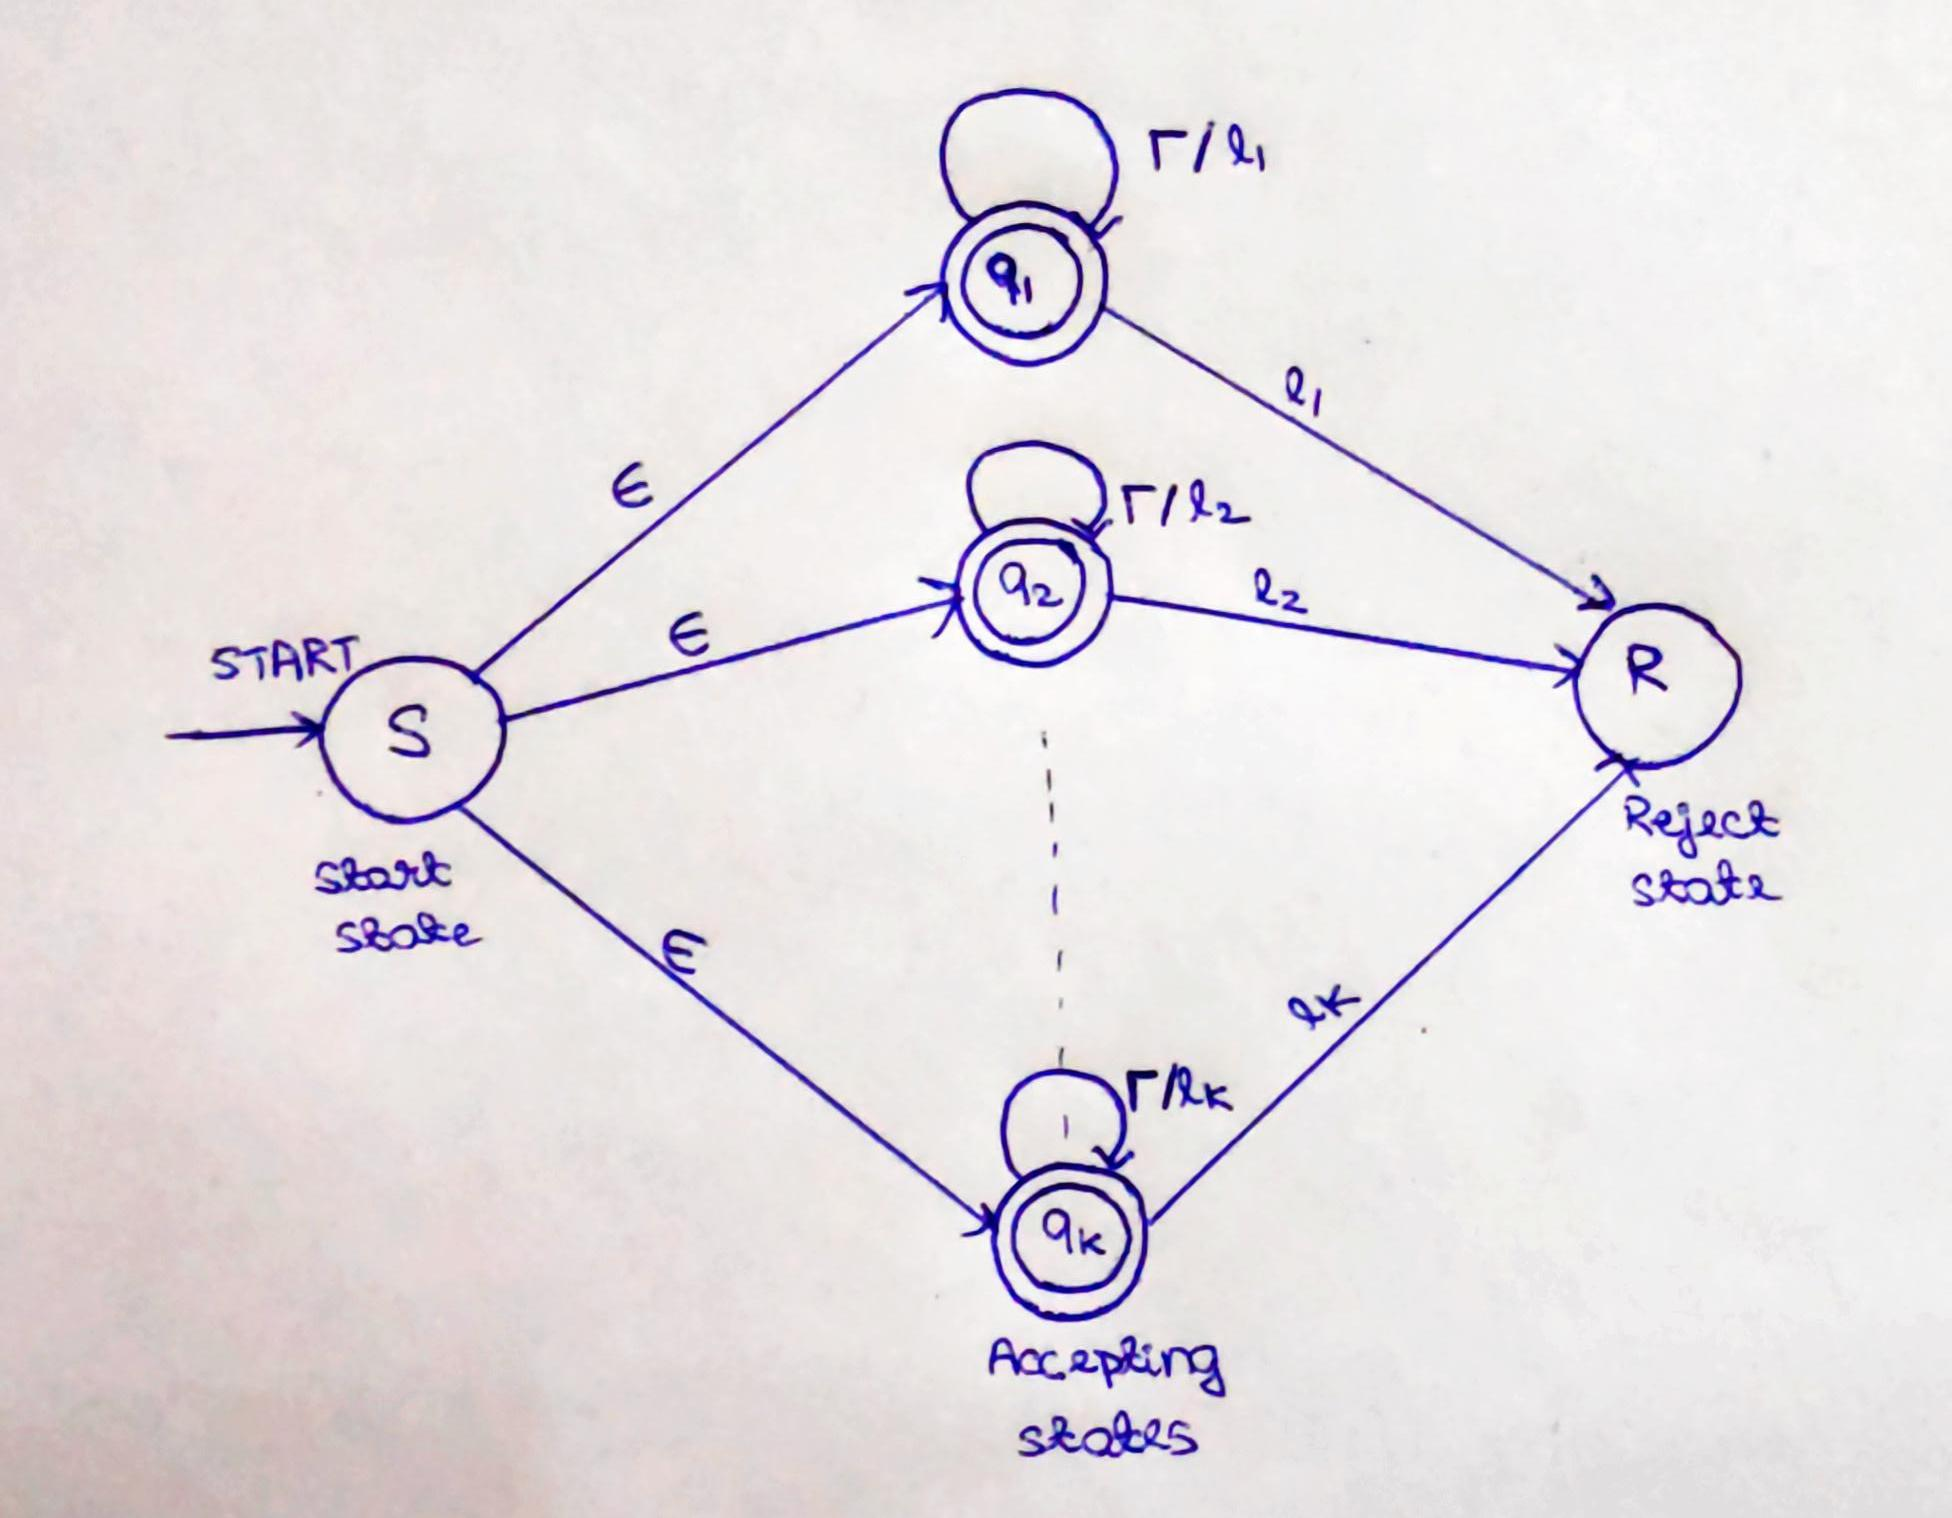
\includegraphics[width=0.7\linewidth]{nfa.jpg}% here goes the figure name
    \caption{NFA Design}
    \label{p6}
    \end{figure}
    
    \item An all-NFA M is a 5-tuple $(Q, \Sigma, \delta, q_0, F)$ that accepts $x \in \Sigma^*$ if every possible state that M could be in after reading input x is a state from F. Note, in contrast, that an ordinary NFA accepts a string if some state among these possible states is an accept state. Prove that all-NFAs recognize the class of regular languages.
    
    \clearpage
    \textbf{Solution:}
    
    We have to prove that the language recognized by all-NFAs is regular. Take an arbitrary all-NFA $N$. Modify $N$ by adding a reject state which is the target of every transition that isn't defined in $N$. The resulting all-NFA is $N_1$. The language recognized by $N_1$ and $N$ is same as only transitions that weren't defined are sent to a reject state. Generate $N_2$ where $N_2$ is same as $N_1$ except the accept states are now non-accept states and the non-accept states are now accept states. Define $N_2$ as a standard NFA instead of all-NFA. \\
    
    \textit{Claim:} L($N_2$) is complement of L($N_1$)\\
    \textit{Proof:} Proof by cases\\
    Take a arbitrary input string $W_1$.\\
    \textit{Case 1:} $W_1$ is accepted by $N_1$\\
    This implies that all the paths in $N_1$ go to a accepting state. In $N_2$, all those end states are reject states as it is opposite. This means, $N_2$ can't accept $W_1$ as all the paths go to a reject state in $N_2$.\\
    
    \textit{Case 2:} $W_1$ is rejected by $N_1$\\
    This implies there exists atleast one run R in $N_1$ that goes to a reject state S in $N_1$. This means, in $N_2$, in the run R, S is a accepting state (opposite of $N_1$). This means $W_1$ is accepted by $N_2$.\\
    
    This proves that L($N_2$) is complement of L($N_1$). As $N_2$ is a standard NFA, L($N_2$) is regular (by definition). Since complement of regular languages are also regular (discussed in lecture), L($N_1$) is also regular. As L($N_1$) = L($N$) by construction, language accepted by arbitrary all-NFA is also regular. Hence proved. 
    
    
    
    \item Show that regular languages are closed under the \textbf{repeat} operation, where \textbf{repeat} operation on a language L is given  \begin{center}
    {\textbf{repeat}(L) = $\{l_1l_1l_2l_2...l_kl_k$ $|$ $ l_1l_2...l_k \in L\}$}
    \end{center}
    
    \textbf{Solution:}
    
    Since $L$ is a regular language $\exists$ DFA $A$ $=$ ($Q$, $\Sigma$, $q_0$, $F$, $\delta$) which recognizes $L$.
    To show that regular languages are closed under the repeat operation, we are required to show that $L'$ is recognized by some NFA $A'$.
    
    $A'$ can be obtained from $A$ by the following constructions:
    
    For every arc from a state $q_i$ to $q_j$ in $A$ insert another state $q_{ij}$ in $A$ such that the arc goes through the newly added state $q_{ij}$ i.e if the transition in $A$ is defined as $\delta (q_i, l_i)$ $=$ $q_j$. Then add $q_{ij}$ and replace the transition $\delta (q_i, l_i)$ $=$ $q_j$ by the transitions $\delta' (q_i, l_i)$ $=$ $q_{ij}$ and $\delta' (q_{ij}, l_i)$ $=$ $q_j$ to obtain $A'$. So $A'$ $=$ $(Q', \Sigma, q_0, F, \delta')$.
    
    \textbf{Correctness}:
    
     \underline{Claim}: If a string $w$ $=$ $l_1l_2...l_k$ is accepted by A then $w'$ $=$ $l_1l_1l_2l_2...l_kl_k$ is accepted by $A'$.
        
        If $w$ is accepted by $A$ then $\exists$ a run of the automaton $p_0p_1...p_n$ s.t 
        $p_0$ $=$ $q_0$ and $p_n$ $\in$ $F$. In obtaining $A'$ from $A$ we had only added few more states and modified the transition function. Leveraging that fact we can show that $w'$ will be accepted by $A'$. Consider the run of automaton $A'$ $p_0p_1....p_n$. We know from the construction that if $\delta (p_i, l_i)$ $=$ $p_j$ then $\delta' (p_i, l_i)$ $=$ $p_{ij}$ and $\delta' (p_{ij}, l_i)$ $=$ $p_j$. So if $l_i$ caused the transition from $p_i$ to $p_j$ in $A$ then $l_i$ will cause the transition from $p_i$ to $p_j$ in $A'$. We can see from this correspondence that $w'$ will be accepted by $A'$.\\
        It can be similarly shown that if $w$ is rejected by $A$ then $w'$ will be rejected by $A'$
    
    
    \item Design an algorithm that takes as input the descriptions of two DFAs, $D_1$ and $D_2$, and determines whether they recognize the same language.
    
    \textbf{Solution:}
    
    Given two DFAs $D_1$ and $D_2$ we are required to design an algorithm which determines whether they recognize the same language i.e are equivalent or not. Now, the DFA $D_1$ and $D_2$ are equivalent iff $L(D_1)$ $\subseteq$ $L(D_2)$ and vice versa. This condition can be restated by using intersection and complement operations which is,  $D_1$ and $D_2$ are equivalent iff 
    \begin{center}
    $\overline{L(D_1)}$ $\cap$ $L(D_2)$ $=$ $\phi$ and $L(D_1)$ $\cap$ $\overline{L(D_2)}$ $=$ $\phi$
    \end{center}
    
    The algorithm for determining whether $D_1$ is equivalent to $D_2$ or not is as follows:
    
    \textbf{Step-1}: Obtain the DFA which recognizes $\overline{L(D_1)}$ by doing the following constructions:
    
    \begin{enumerate}
        \item Make every accepting state in $D_1$ rejecting state.
        \item Make every rejecting state in $D_1$ accepting state.
    \end{enumerate}
    
    \textbf{Step-2}: Obtain the DFA which will recognize $\overline{L(D_1)}$ $\cap$ $L(D_2)$. In Step-1 we have obtained the DFA which recognizes $\overline{L(D_1)}$. The DFA which recognizes $\overline{L(D_1)}$ $\cap$ $L(D_2)$ then can be constructed using product construction.
    
    \textbf{Step-3}: We have the DFA which recognizes $\overline{L(D_1)}$ $\cap$ $L(D_2)$. Now checking if $\exists$ a path from a start state to an accepting state will determine whether $\overline{L(D_1)}$ $\cap$ $L(D_2)$ is an empty set or not. If there does not exist any path from a start state to an accepting state in the DFA then it is empty otherwise not.
    
    \textbf{Step-4}: If the DFA in Step-3 does not contain a path from a start state to an accepting state then repeat Step-1, 2, 3 for $L(D_1)$ $\cap$ $\overline{L(D_2)}$ else $D_1$ and $D_2$ are not equivalent. 
    
    \textbf{Step-5}: If $L(D_1)$ $\cap$ $\overline{L(D_2)}$ also turn out be an empty set then $D_1$ and $D_2$ are equivalent otherwise they are not.

    
    
    
    \item For any string $w = w_1w_2...w_n$ the reverse of $w$ written $w^R$ is the string $w_n...w_2w_1$. For any language $A$, let $A^R$ = $\{w^R \,|\, w \in A\}$. Show that if $A$ is regular, then so is $A^R$. In other words, regular languages are closed under the reverse operation.
    
    \textbf{Solution:}
    
    If A is regular, there exists DFA X that accepts A.
    Let X = (Q1, $\Sigma$, q0, F1, $\delta$1)
    
    Let q1 = dummy start state\\
    Create NFA Y such that,\\
    
    Y = (Q1 + q1, $\Sigma$, q1, q0, $\delta$2), where $\delta$2 = reverse of all transitions in $\delta$1 + $\epsilon$ transition from q1 to all members in F1. \\
    
    To Prove: L(Y) = $A^R$\\
    Proof: Proof by cases\\
    
    Case 1:\\
    Let w1 be an arbitrary string in A. Let $w1^R$ be reverse of w1. \\
    As w1 is in A, the run of w1 ends up in some accept state s0 in X. This s0 is connected to q1 in Y. Thus retracing of that path (reverse) would go to q0 in Y, where q0 is an accept state. This means $w1^R$ is accepted by Y, where $w1^R$ is an arbitrary string in $A^R$. 
    
    Case 2:\\
    Proof by contradiction:
    Let w2 be an arbitrary string that isn't accepted by X. Let $w2^R$ be reverse of w2. \\
    
    Assume $w2^R$ is accepted by Y. \\
    The run of $w2^R$ in Y would start in one of the states s1 in F1, and end at q0 for it to be accepted by Y. The reverse of this run would have the string w2. This implies, w2's run in X would start at q0 and end at s1 in X. This implies w2 is accepted by X, which is a contradiction. This implies that the assumption is wrong. $w2^R$ isn't accepted by Y, where $w2^R$ is an arbitrary string not present in $A^R$. \\
    
    Thus proved, L(Y) = $A^R$\\
    
    As $A^R$ is L(Y), it is accepted by Y NFA. Thus, $A^R$ is a regular language by definition, where A is an arbitrary regular language \\
    
    Therefore, regular languages are closed under the reverse operation.\\
    
    
    \item Let $\Sigma$ and $\Gamma$ be two finite alphabets. A function $f : \Sigma^* \rightarrow \Gamma^*$ is called a homomorphism if for all $x, y \in \Sigma^*, f(x . y) = f(x) . f(y)$. Observe that if $f$ is a string homomorphism, then $f(\epsilon) = \epsilon$, and the values of $f(a)$ for all $a \in \Sigma$ completely determines $f$. Prove that the class of regular languages is closed under homomorphisms. That is, prove that if $L \subseteq \Sigma^*$ is a regular language, then $f(L) = \{f(x) \in \Gamma^* \,|\, x \in L\}$ is regular. Try to informally describe how you will start with a DFA for $L$ and get an NFA for $f(L)$.
    
    \textbf{Solution:}
    
    Regular languages can be represented in terms of regular expressions. For any regular expression $R$,\, $f(L(R)) = L(f(R))$. This can be proved by induction on number of terms in $R$. We need to show the induction for all types of regular expressions- $R_1 \cup R_2$, $R^*$ and $R_1.R_2$. For $R = R_1.R_2$, $f(R_1.R_2) = f(R_1).f(R_2)$ and $f(L(R)) = f(L(R_1).L(R_2)) = f(L(R_1)).f(L(R_2))$. By induction hypothesis, $f(L(R_1)) = L(f(R_1))$ and $f(L(R_2)) = L(f(R_2))$ so, $f(L(R)) = L(f(R_1)).L(f(R_2)) = L(f(R_1.R_2)) = L(f(R))$. Similar arguments can be given for other cases.\\
    The regular language $L$ is written as $L(R)$ where $R$ is some regular expression. Using above property, ${f(L) = f(L(R)) = L(f(R)) = L(R^{'} )}$. Thus, $f(L)$ can be represented as the language of some regular expression $R^{'}$ which is regular.\\
    The NFA of $f(L)$ can be constructed by replacing every letter $a$ in the original DFA by $f(a)$. This will be a NFA because there may be elements in $\Gamma^*$ which are not mapped to elements in $\Sigma^*$. 
    
\end{enumerate}

\end{document}
